\begin{anexosenv}
\partanexos
\chapter{Primeiro Anexo}
A figura abaixo se refere a primeira parte do modelo de contrato usado na empresa.
\begin{figure}[h!]
    \centering
    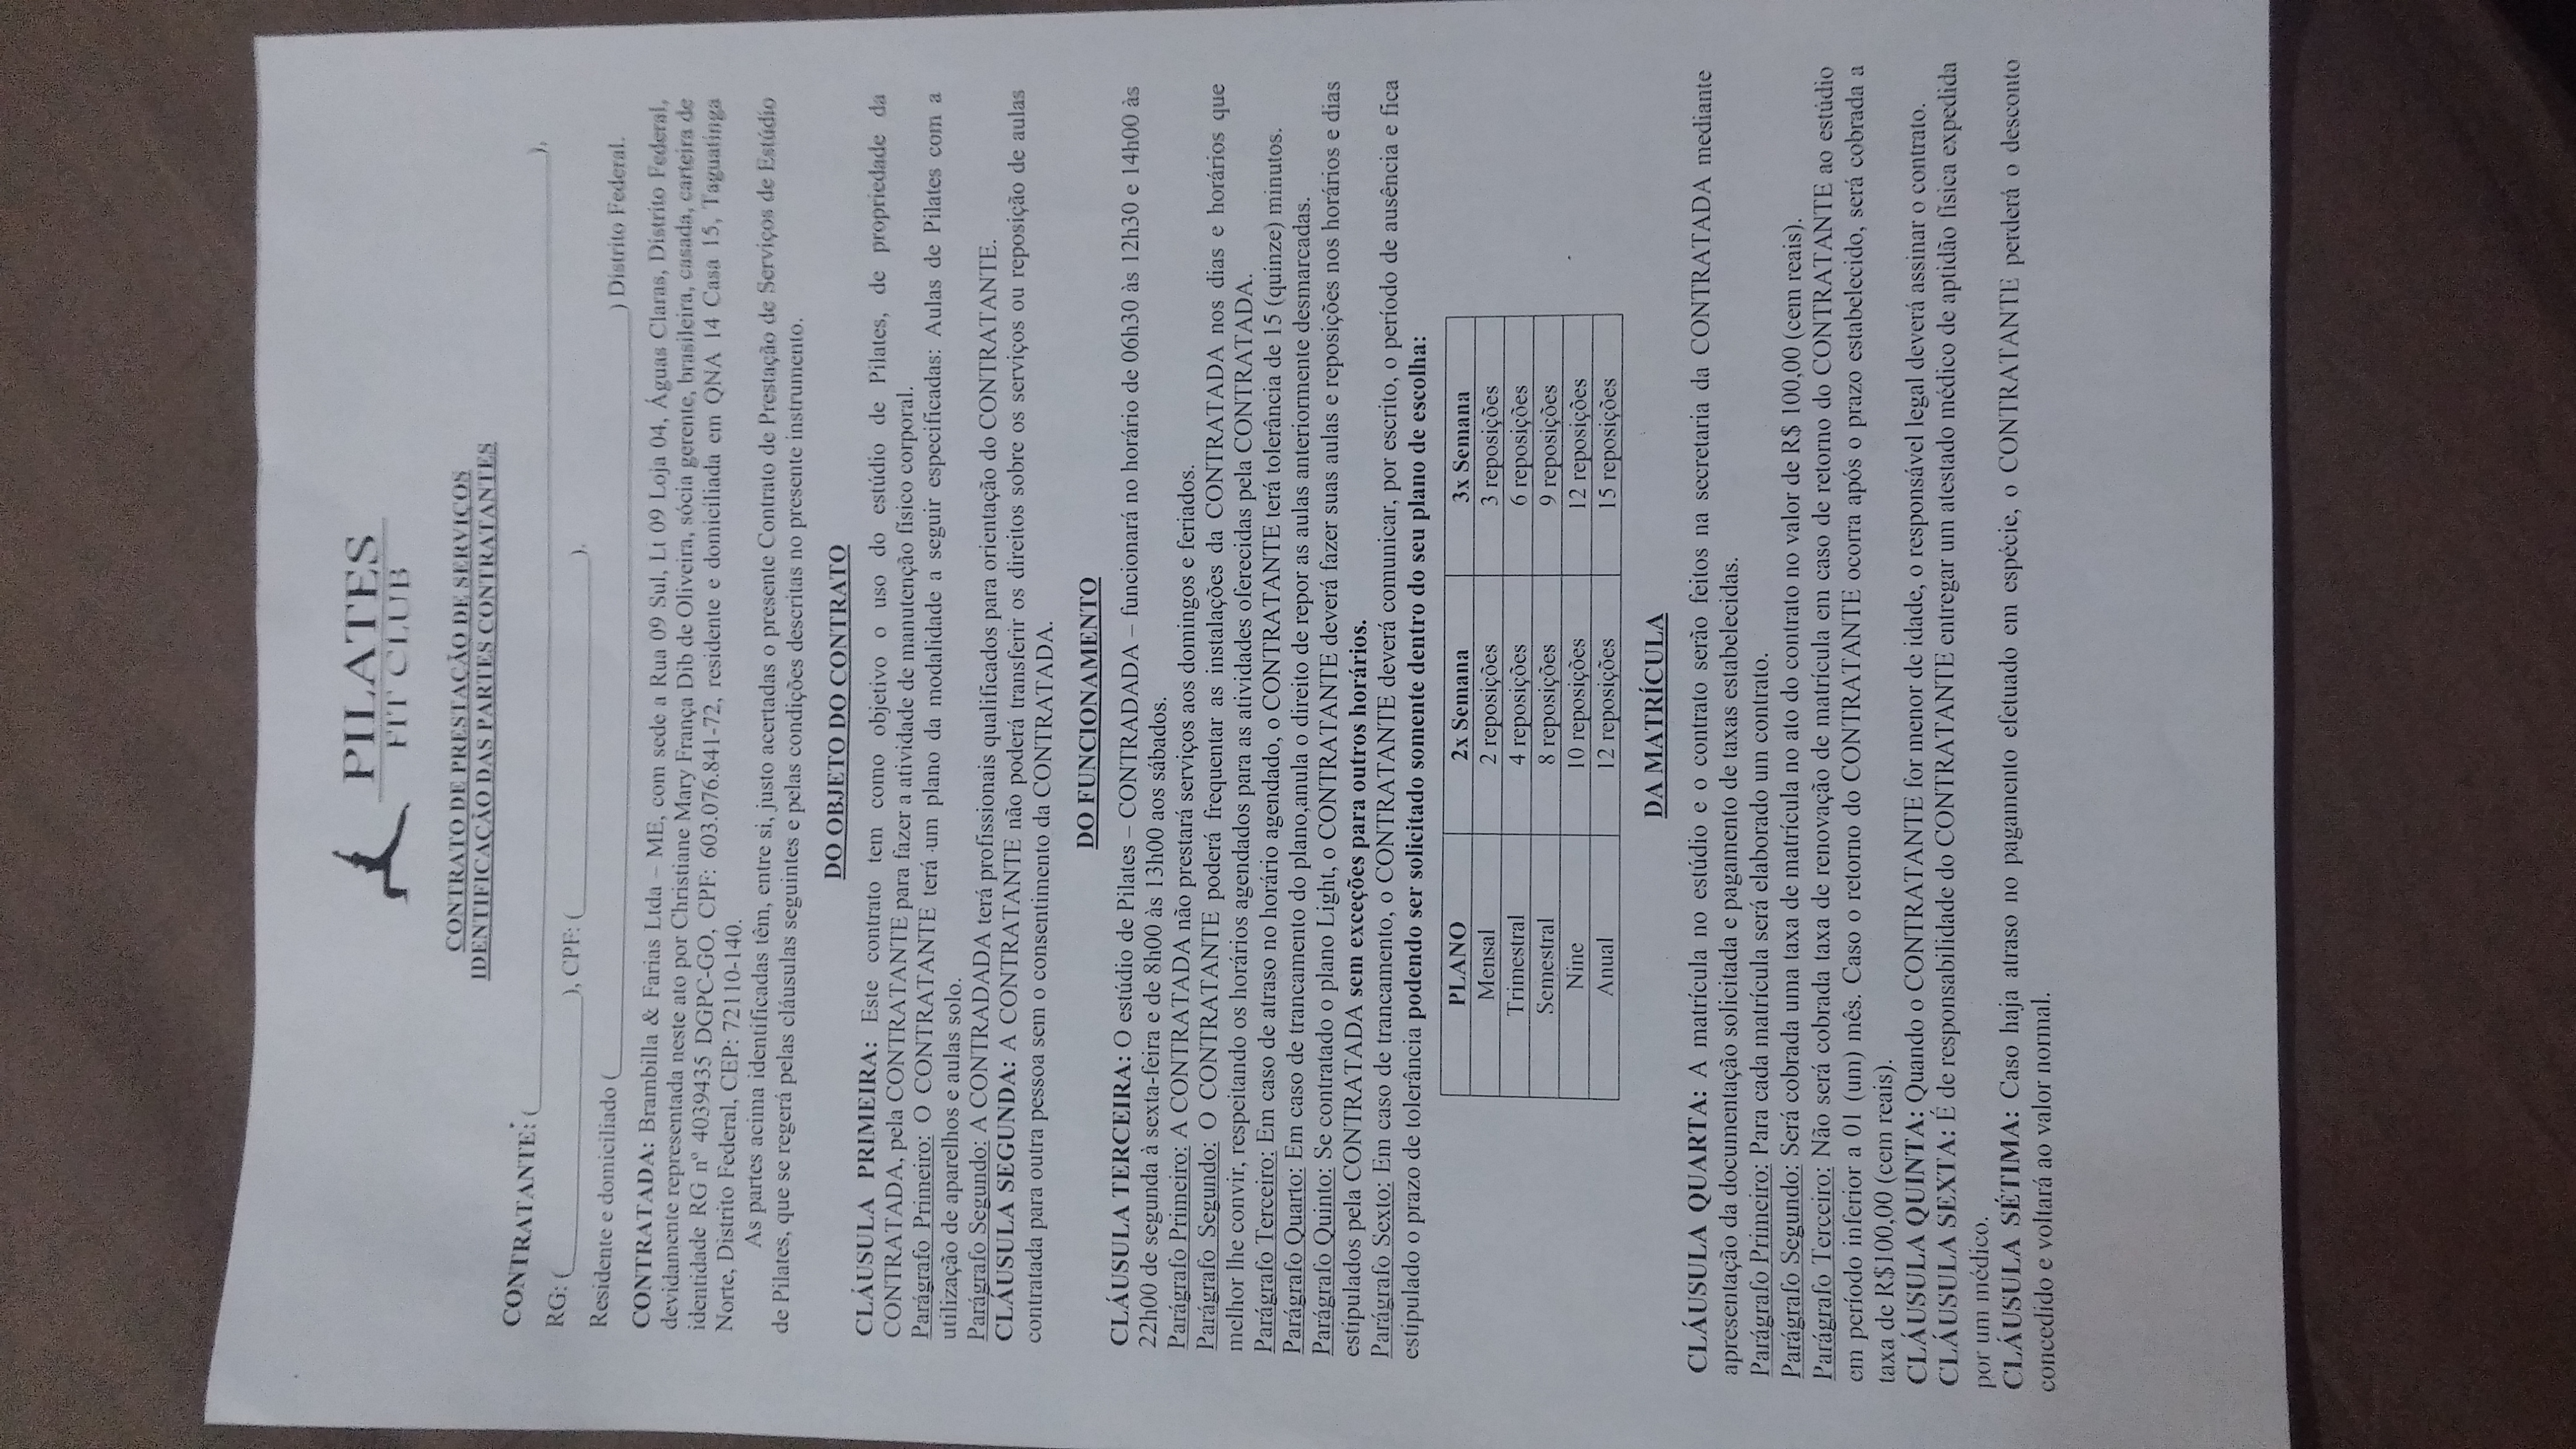
\includegraphics[width=\textwidth, angle=-90]{figuras/contrato_1.jpg}
    \caption{Plano de Contrato, página 1.}
    \label{fig:contrato_1}
\end{figure}
\chapter{Segundo Anexo}
A figura abaixo se refere a segunda parte do modelo de contrato usado na empresa.
\begin{figure}[h!]
    \centering
    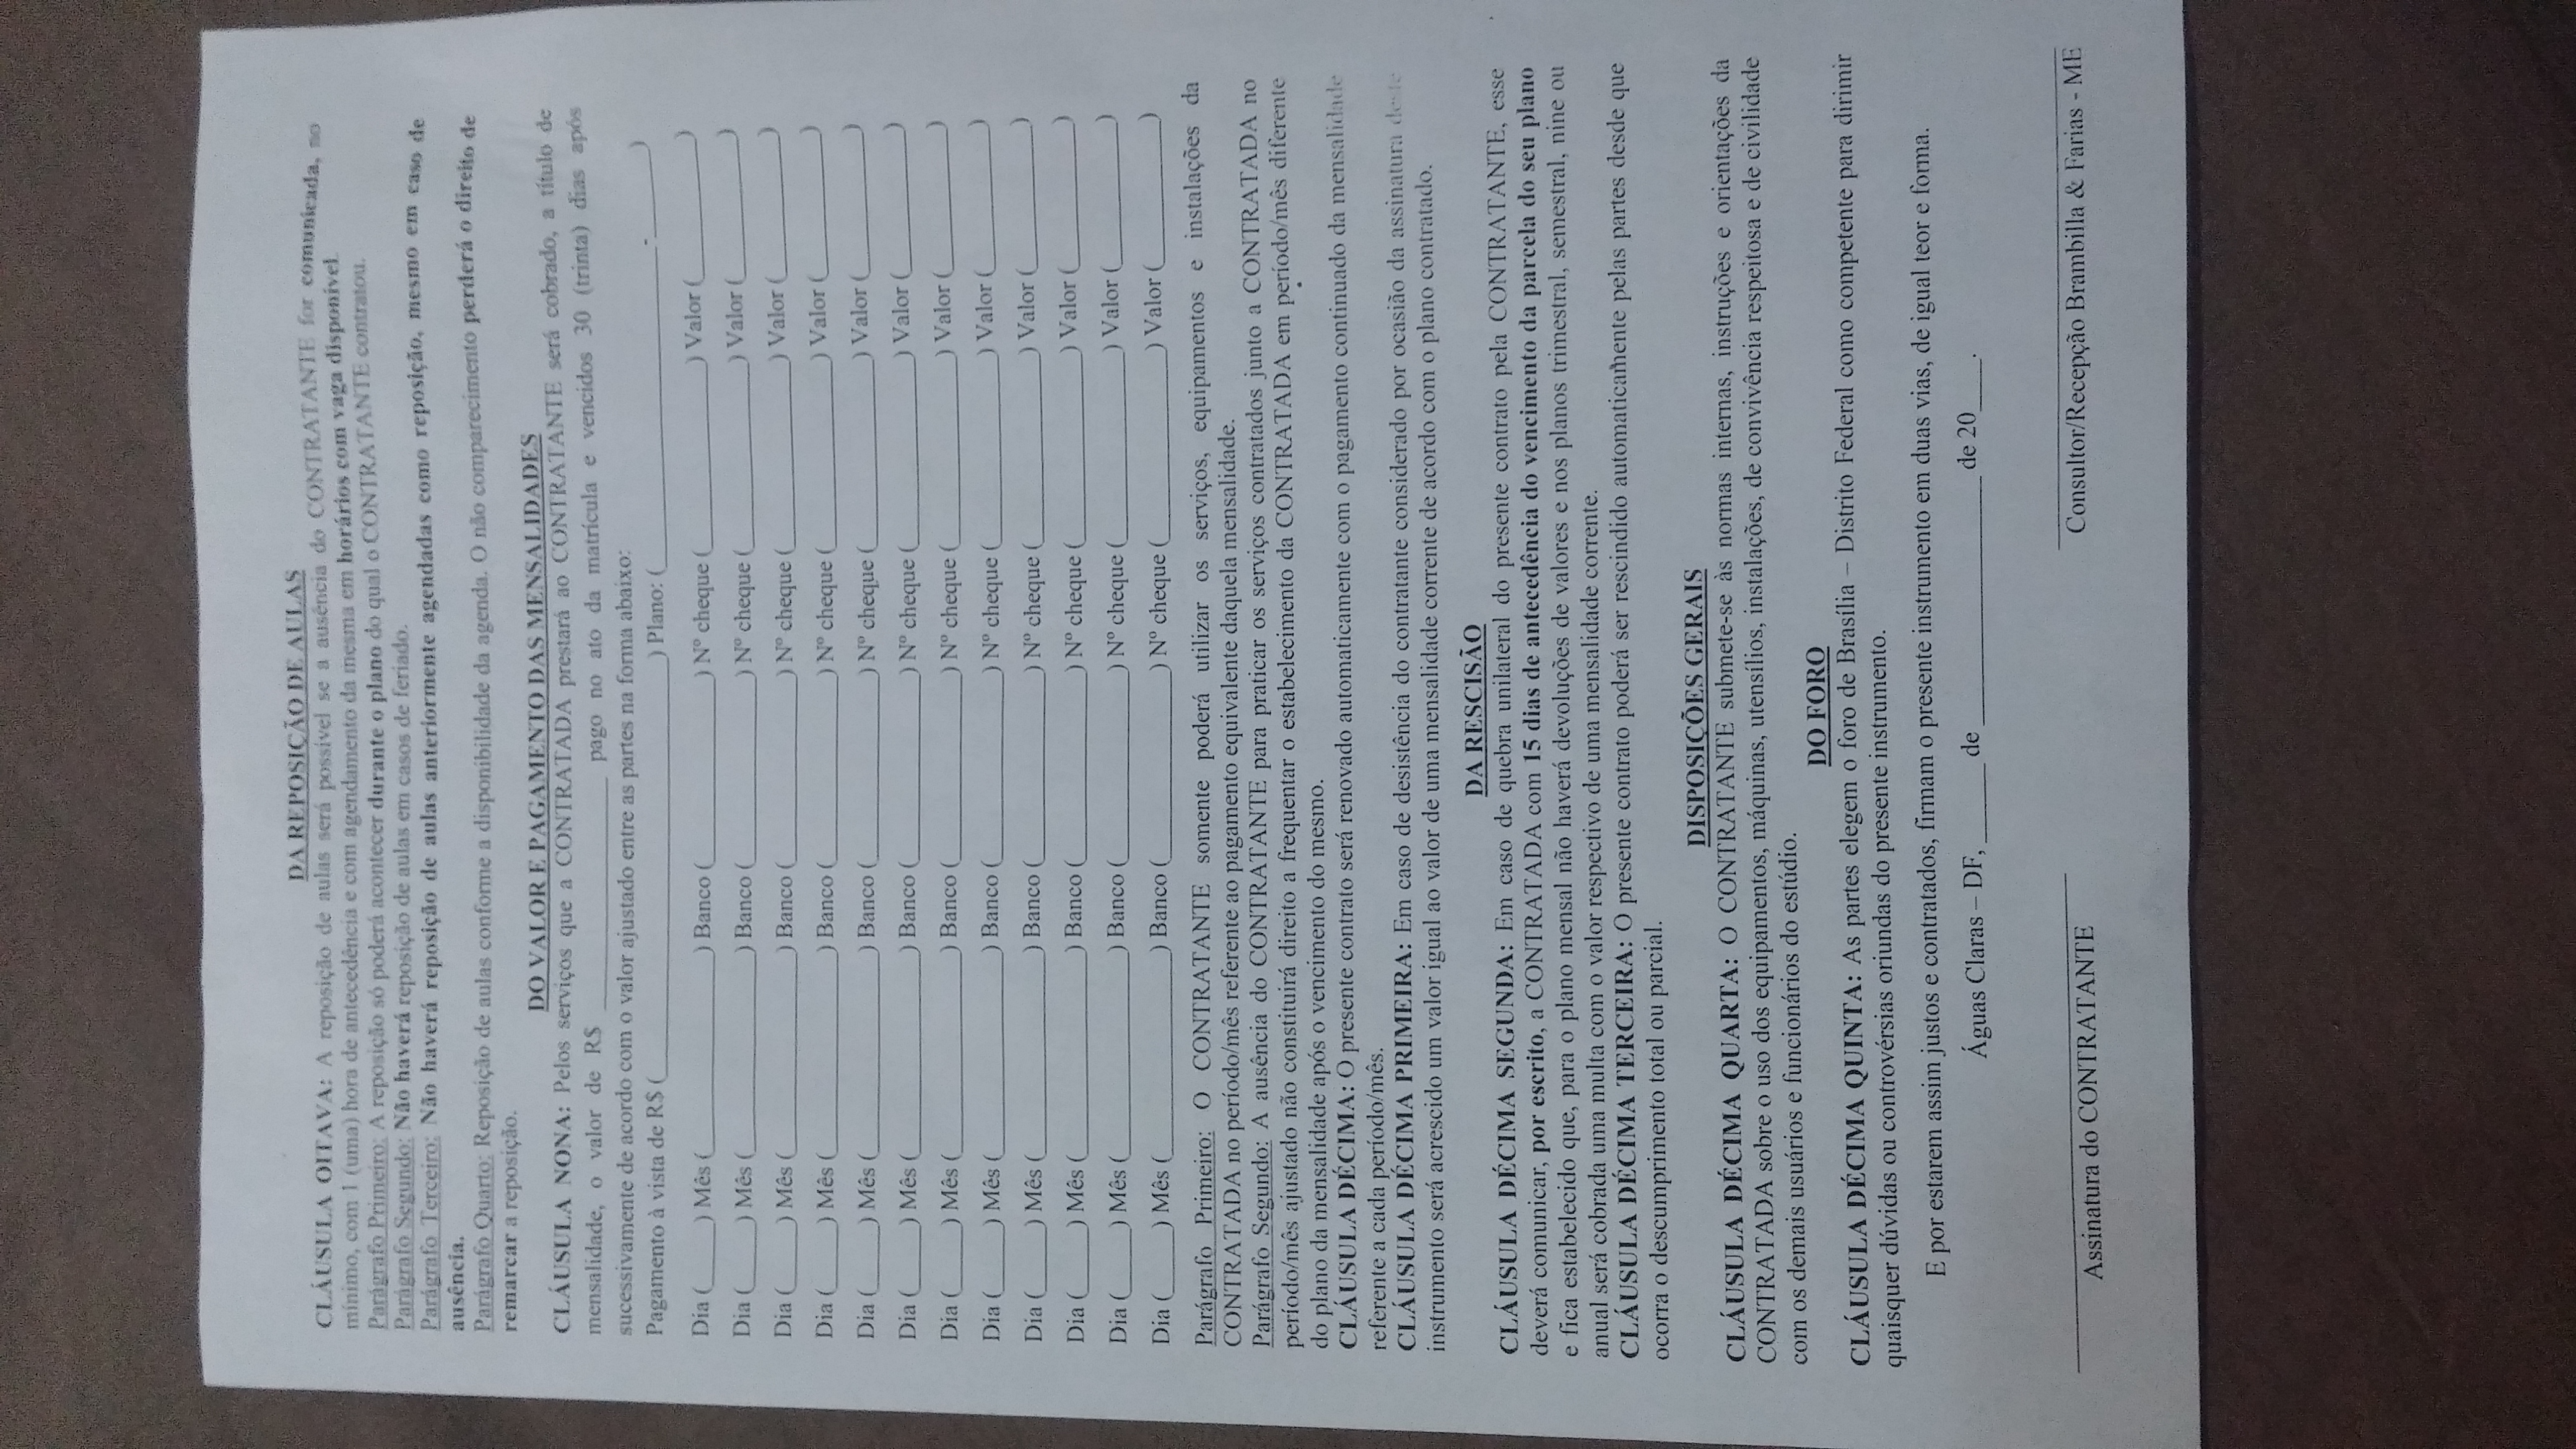
\includegraphics[width=\textwidth, angle=-90]{figuras/contrato_2.jpg}
    \caption{Plano de Contrato, página 2.}
    \label{fig:contrato_2}
\end{figure}
\chapter{Terceiro Anexo}
Esse anexo se refere a ficha de matrícula que a empresa utiliza.
\begin{figure}[h!]
    \centering
    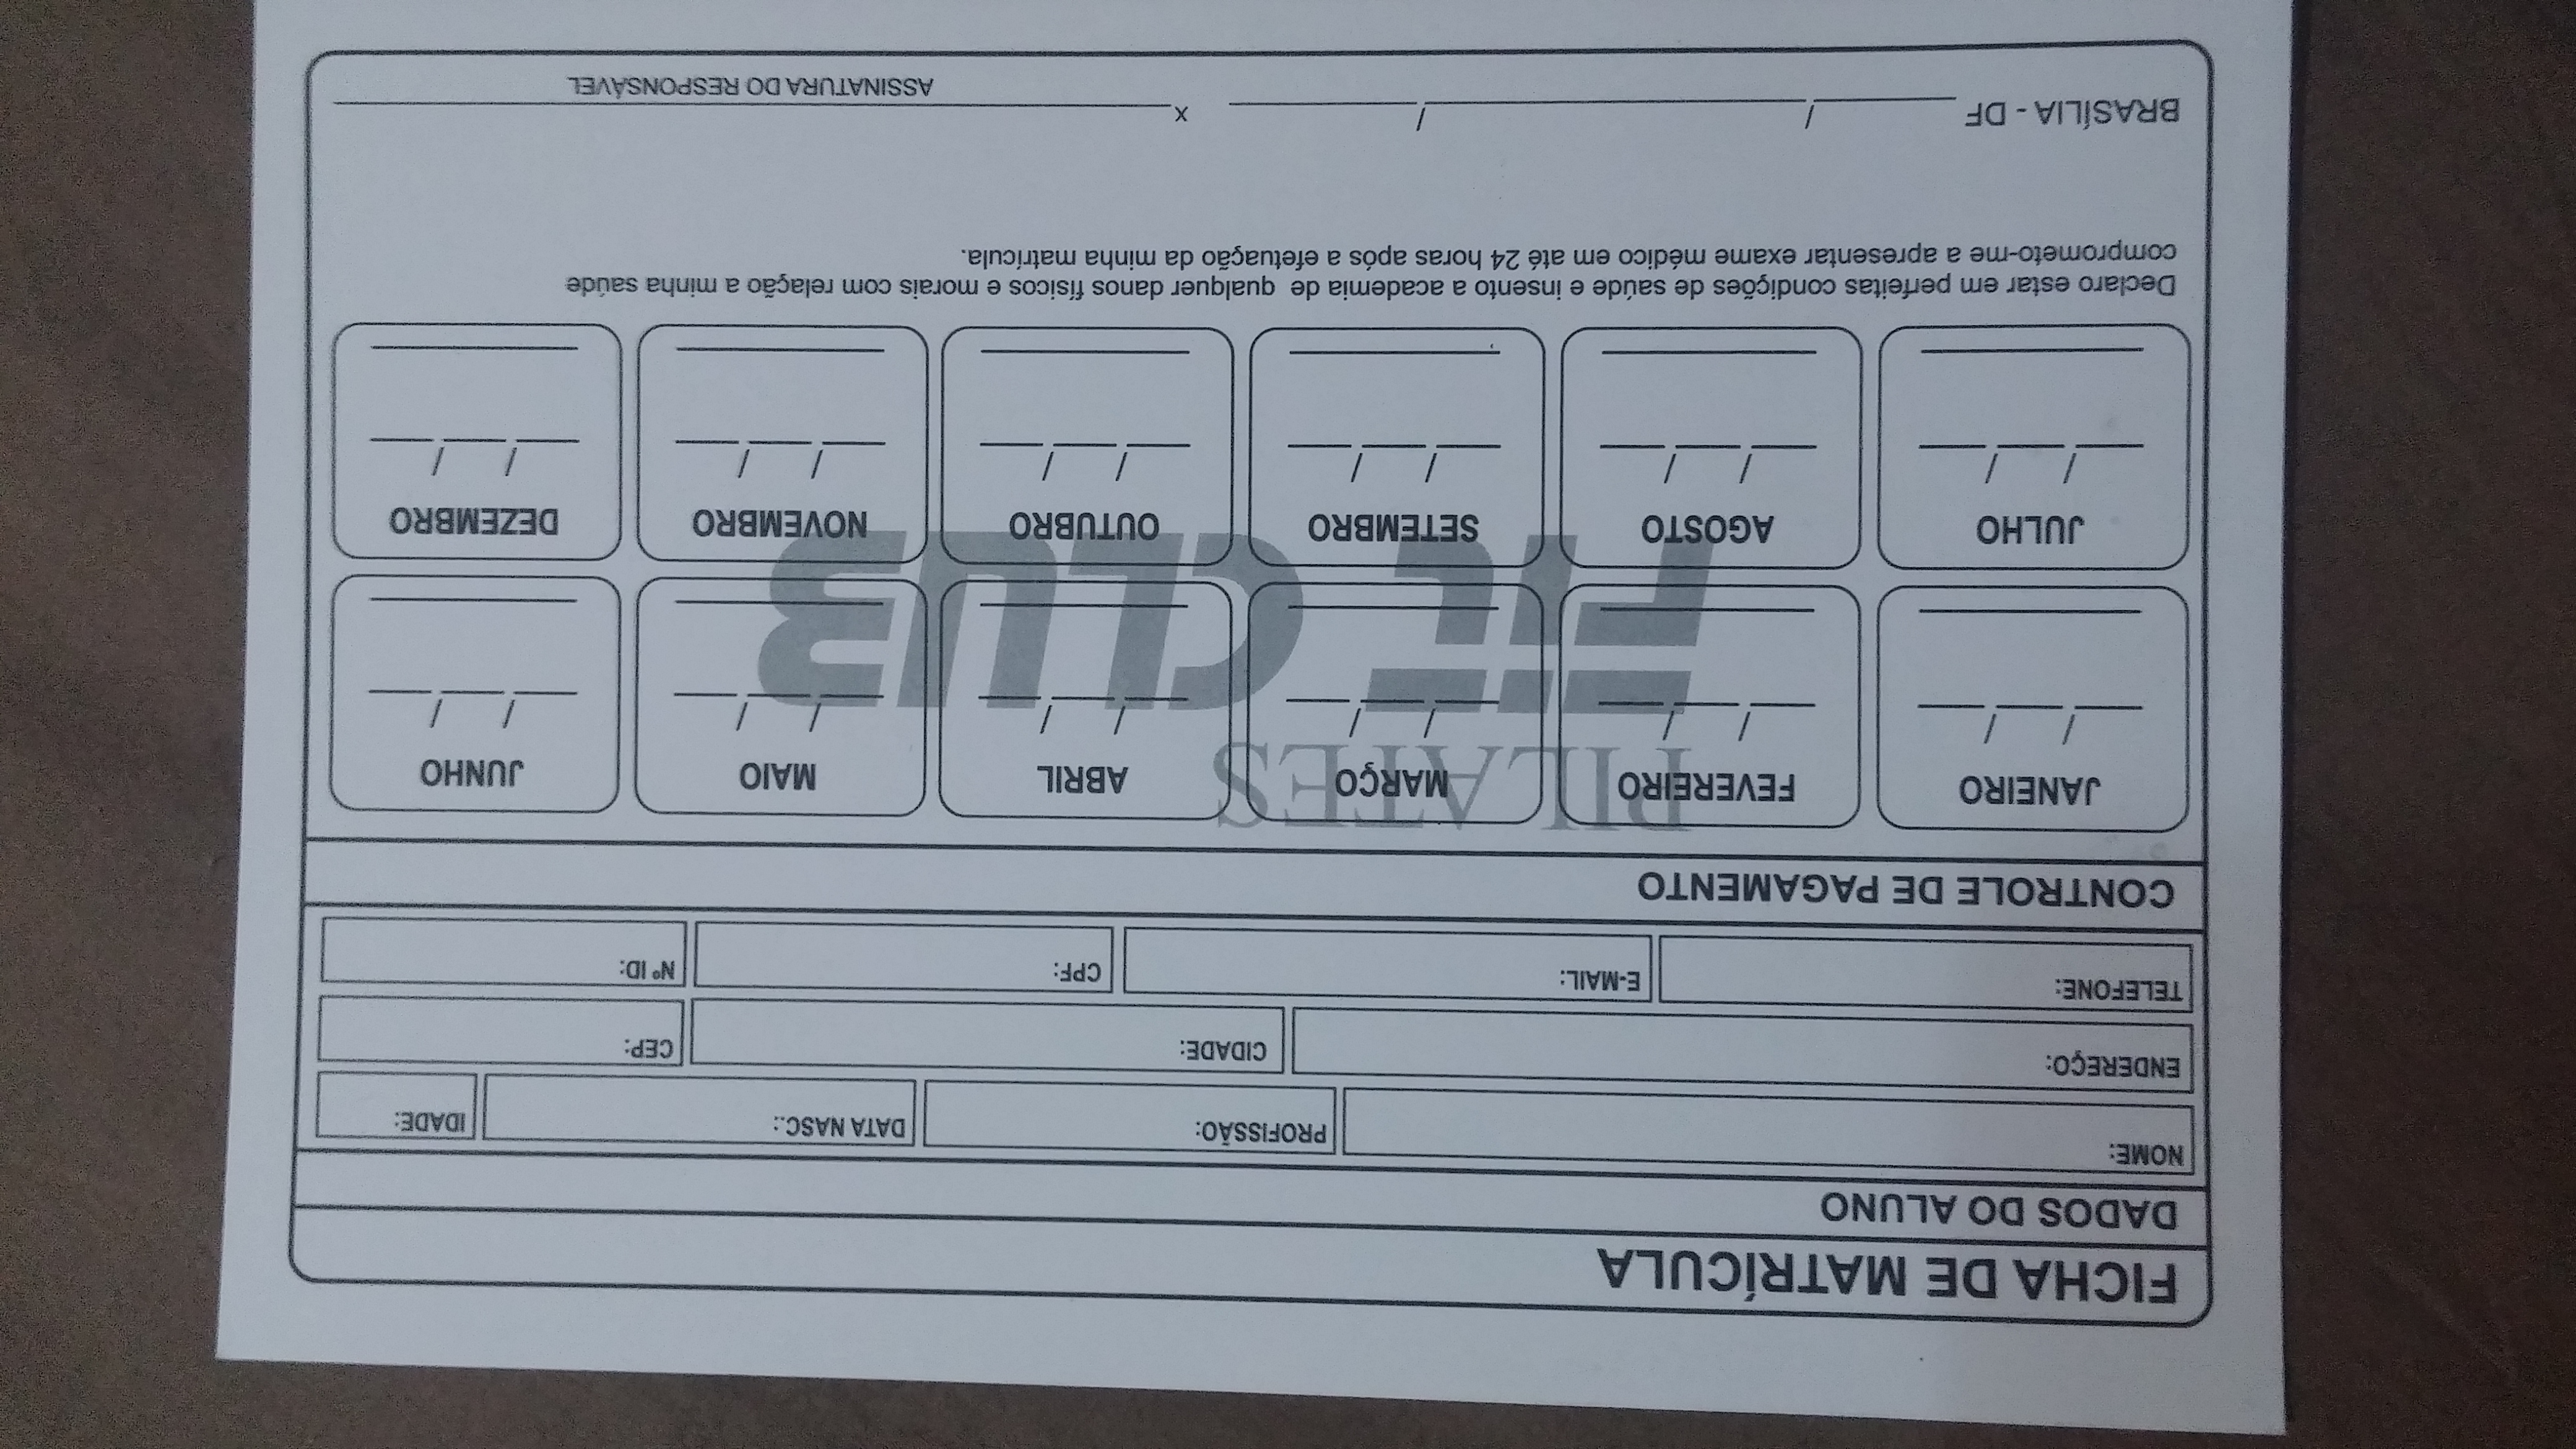
\includegraphics[width=\textwidth, angle=-90]{figuras/matricula.jpg}
    \caption{Ficha de matrícula.}
    \label{fig:matricula}
\end{figure}
\chapter{Quarto Anexo}
Esse anexo mostra como é feito o controle de vencimentos na empresa.
\begin{figure}[h!]
    \centering
    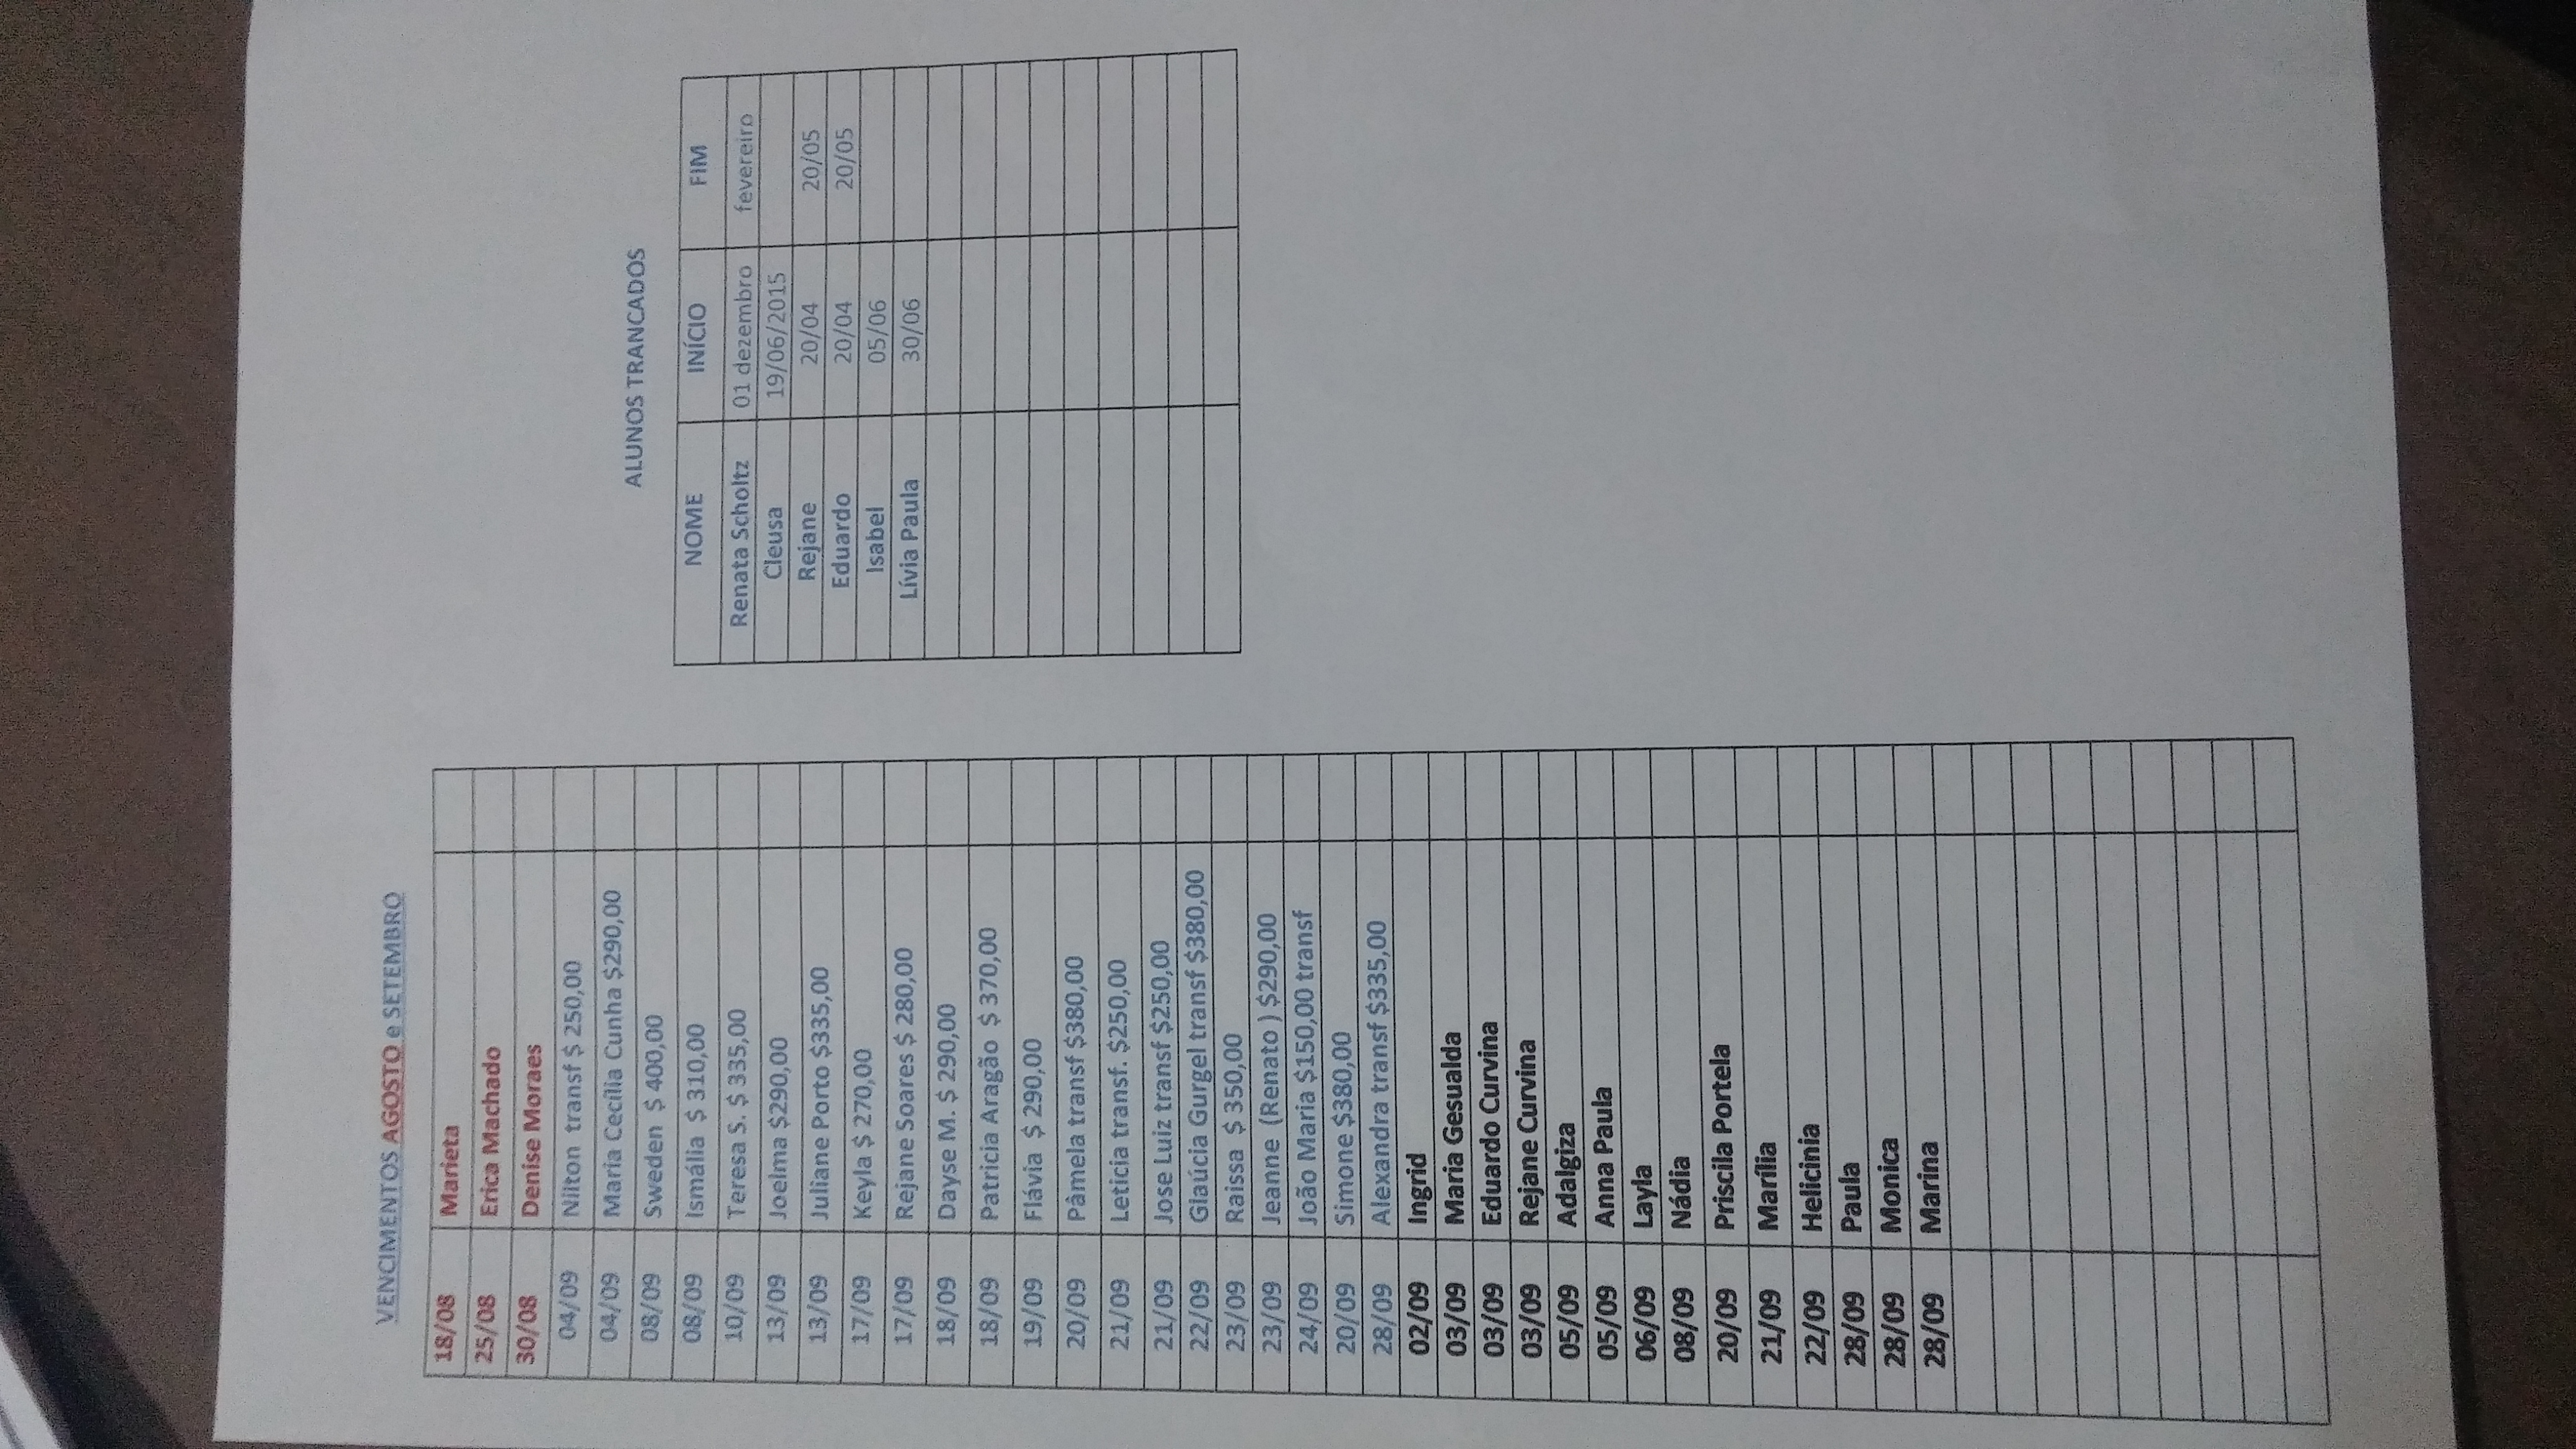
\includegraphics[width=\textwidth, angle=-90]{figuras/vencimentos.jpg}
    \caption{Tabela de vencimentos.}
    \label{fig:vencimentos}
\end{figure}
\end{anexosenv}
